%-------------------------------------------------------
\section{O que é Docker?}
%-------------------------------------------------------

\subsection{Docker vs VM}
\begin{frame}{Docker}{Docker vs VM}
  \begin{figure}[ht!]
    \centering
    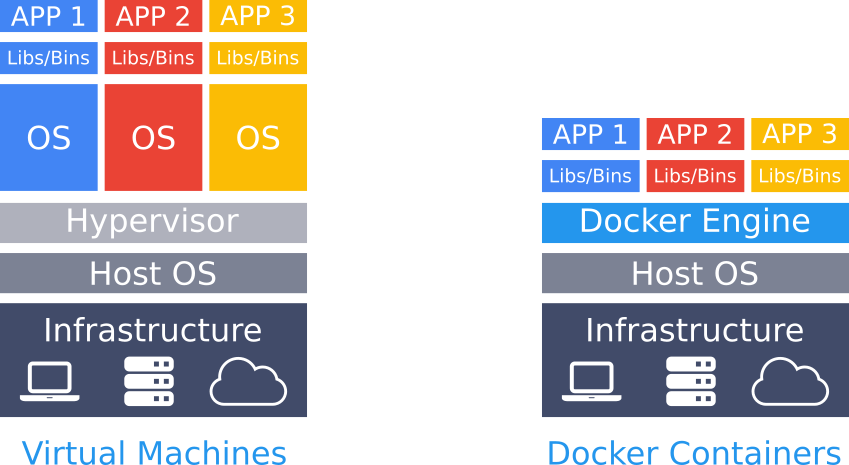
\includegraphics[width=90mm]{images/vm_docker.png}
  \end{figure}
  A finalidade de uma VM é emular totalmente um ambiente, enquanto que a de um contêiner é tornar os aplicativos portáveis e independentes.
\end{frame}

\begin{frame}{Docker}{Docker vs VM}
  \begin{figure}[ht!]
    \centering
    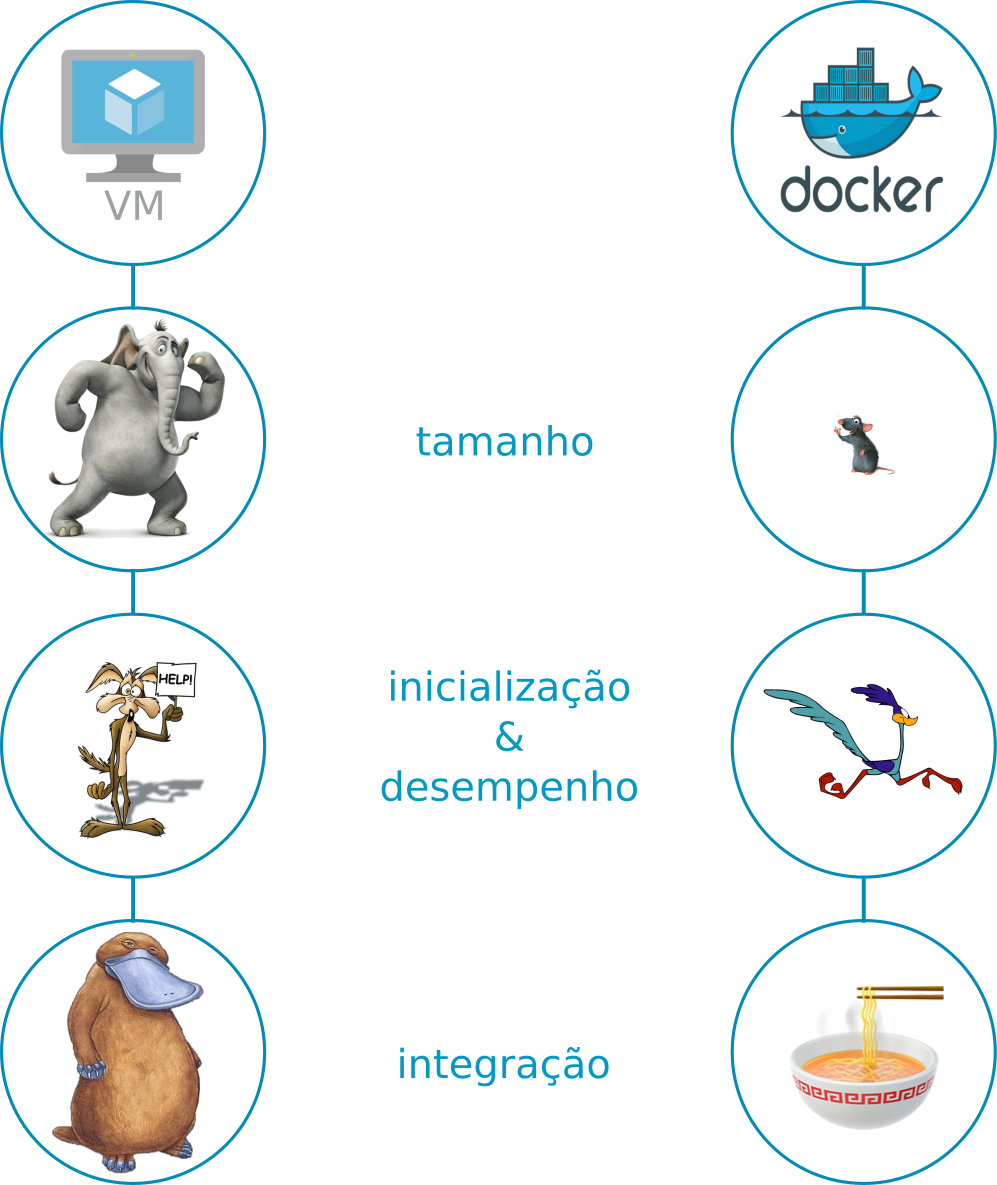
\includegraphics[width=60mm]{images/features.png}
  \end{figure}
\end{frame}

\begin{frame}[fragile]{Docker}{Dockerfile}
  \begin{itemize}
    \item<1-> Dockerfile Correto
  \end{itemize}
  \begin{lstlisting}[language=docker]
  FROM node:10.12.0-alpine

  ADD . /usr/src/app

  WORKDIR /usr/src/app

  RUN npm set progress=false && npm install && npm cache clean --force

  EXPOSE 3000

  ENV HTTP_PORT=9090

  CMD ["npm", "start"]
  \end{lstlisting}
  \begin{lstlisting}[language=bash]
  # bash console
  docker image build -t minha_primeira_imagem:share .
  \end{lstlisting}
\end{frame}

\begin{frame}[fragile]{Docker}{Dockerfile}
  \begin{itemize}
    \item<1-> Dockerfile Incorreto
  \end{itemize}
  \begin{lstlisting}[language=docker]
  FROM node:10.12.0-alpine

  RUN mkdir -p /usr/src/app

  WORKDIR /usr/src/app

  COPY . /usr/src/app

  RUN npm set progress=false

  RUN npm install

  RUN npm cache clean --force

  EXPOSE 3000

  ENV HTTP_PORT=9090

  CMD ["npm", "start"]
  \end{lstlisting}
  \begin{lstlisting}[language=bash]
  # bash console
  docker image build -t minha_primeira_imagem:share .
  \end{lstlisting}
\end{frame}



\subsection{Docker Image}
\begin{frame}{Docker}{Docker Image}
  \begin{figure}[ht!]
    \centering
    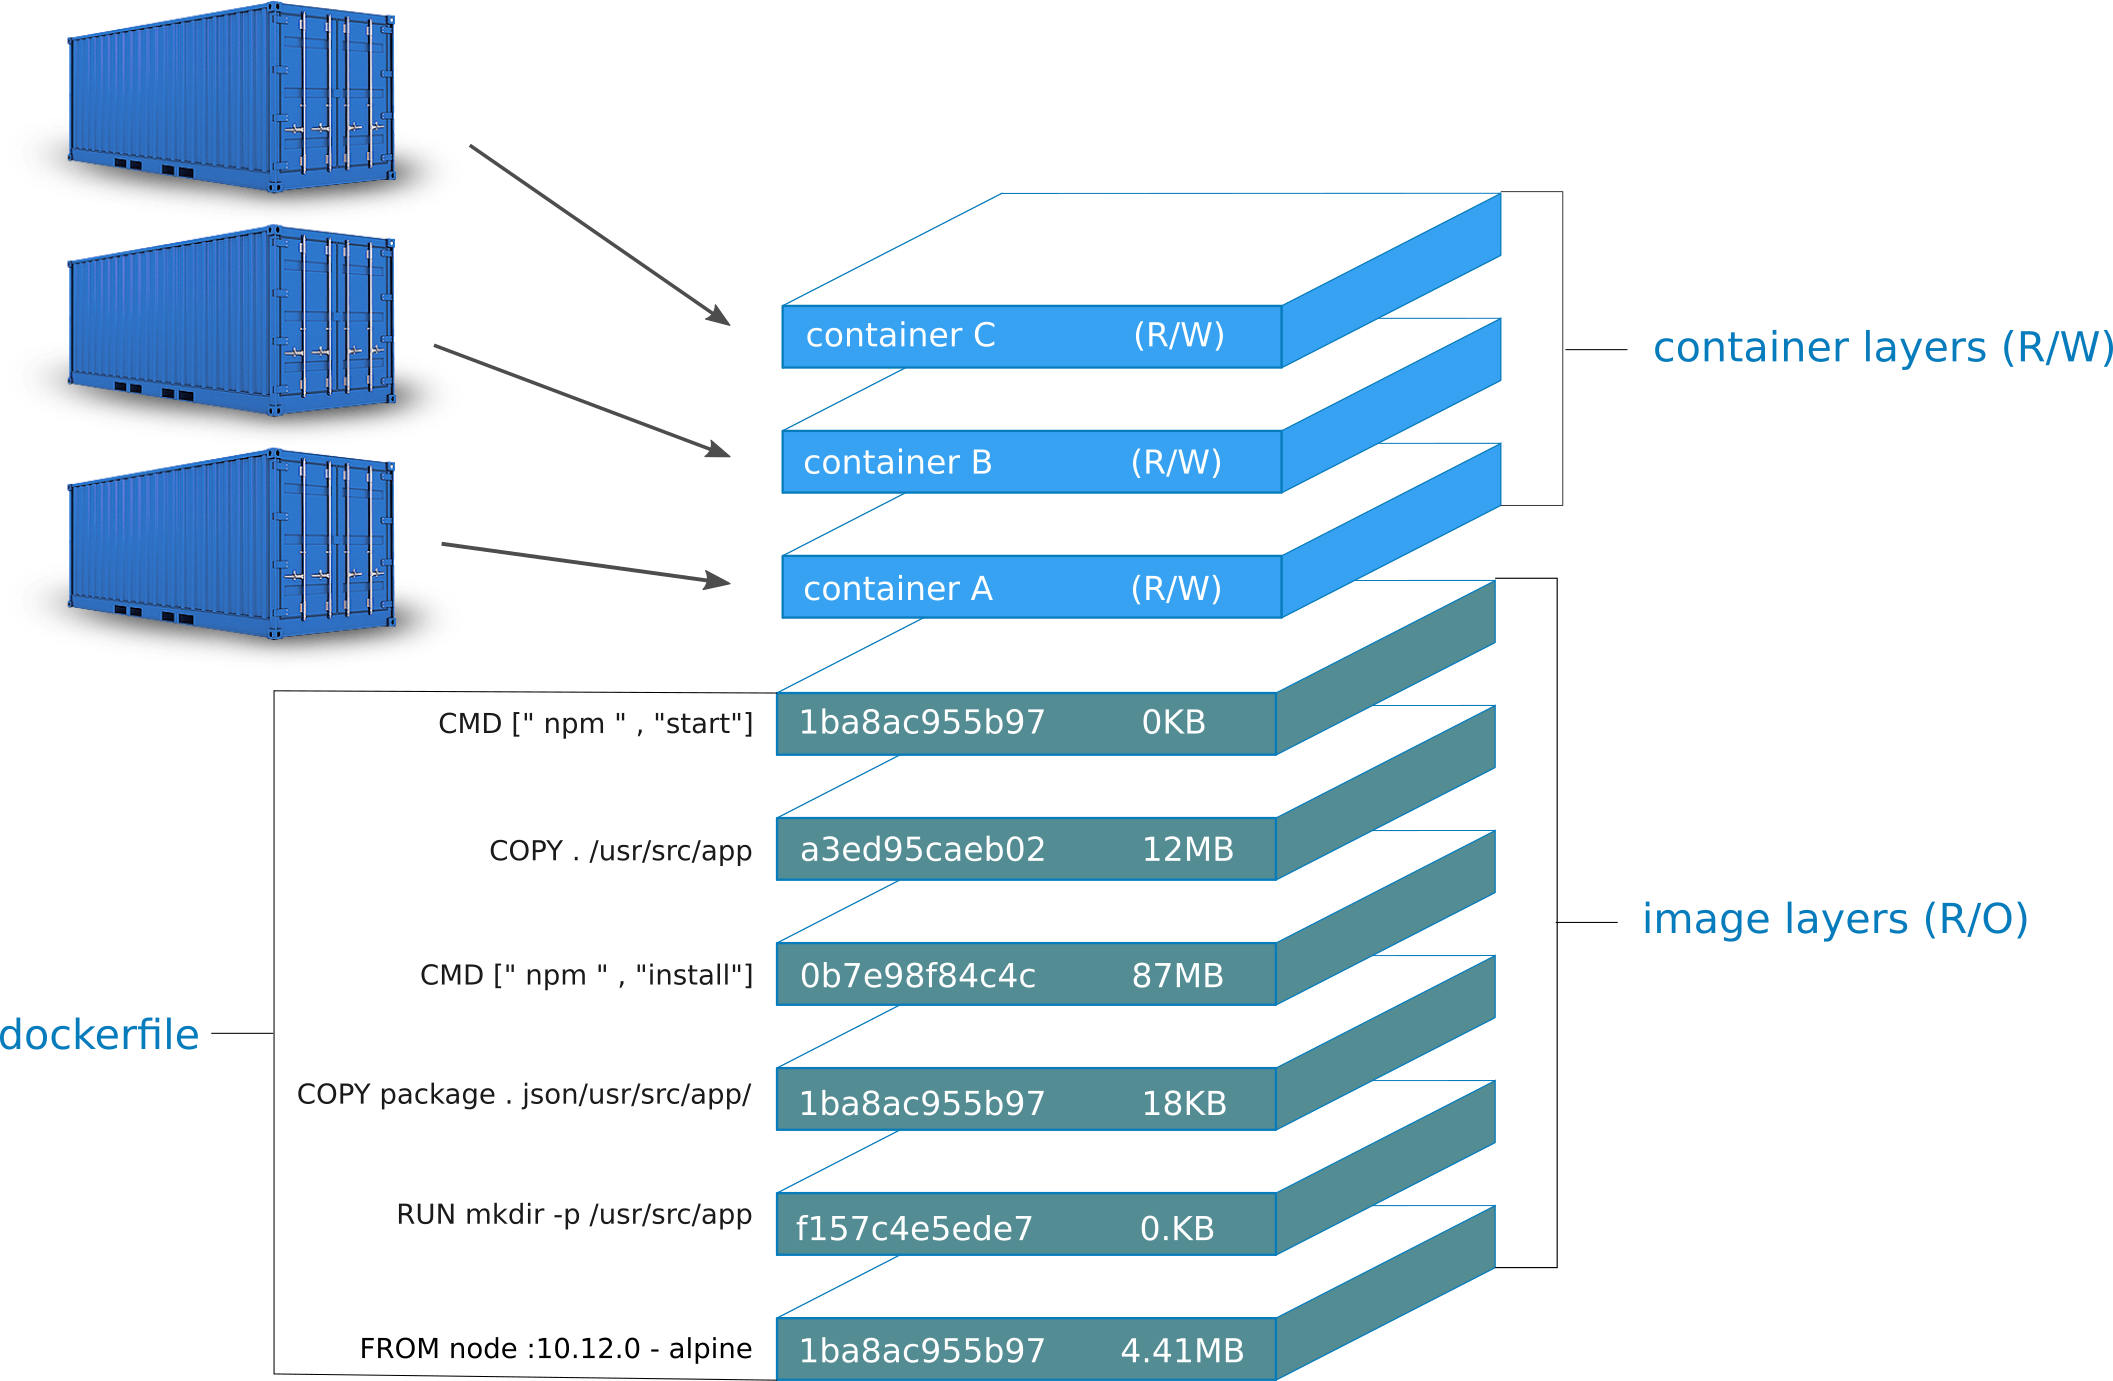
\includegraphics[width=80mm]{images/image.png}
  \end{figure}
  A imagem Docker é um modelo somente leitura a partir do qual os contêineres são instanciados. Cada imagem consiste em uma série de camadas (layers).
\end{frame}
